\documentclass[conference]{IEEEtran}
\usepackage[top=3cm, bottom=2cm, left=2cm, right=2cm, columnsep=20pt]{geometry}
\usepackage{pdfpages}
\usepackage{graphicx}
\usepackage{etoolbox}
\apptocmd{\sloppy}{\hbadness 10000\relax}{}{}
% \usepackage[numbers]{natbib}
\usepackage[T1]{fontenc}
\usepackage{ragged2e}
\usepackage[french]{babel}
\usepackage{listings}
\usepackage{color}
\usepackage{soul}
\usepackage[utf8]{inputenc}
\usepackage[export]{adjustbox}
\usepackage{caption}
\usepackage{mathrsfs, amsmath}
\usepackage{amssymb}
\usepackage{float}
\usepackage{csquotes}
\usepackage{fancyhdr}
\usepackage{wallpaper}
\usepackage{siunitx}
\usepackage[indent]{parskip}
\usepackage{textcomp}
\usepackage{gensymb}
\usepackage{multirow}
\usepackage[hidelinks]{hyperref}
\usepackage{abstract}
\usepackage{subcaption}
\usepackage{tabularx}
\usepackage{biblatex}
\addbibresource{bibliographie.bib}

% \renewcommand{\abstractnamefont}{\normalfont\bfseries}
% \renewcommand{\abstracttextfont}{\normalfont\itshape}
\usepackage{titlesec}
% \titleformat{\section}{\large\bfseries}{\thesection}{1em}{}
% \titleformat{\subsection}{\normalsize\bfseries}{\thesubsection}{1em}{}
% \titleformat{\subsubsection}{\normalsize\bfseries}{\thesubsubsection}{1em}{}

\usepackage{xcolor}
\definecolor{codegreen}{rgb}{0,0.6,0}
\definecolor{codegray}{rgb}{0.5,0.5,0.5}
\definecolor{codepurple}{rgb}{0.58,0,0.82}
\definecolor{backcolour}{rgb}{0.95,0.95,0.92}
\lstdefinestyle{mystyle}{
    backgroundcolor=\color{backcolour},   
    commentstyle=\color{codegreen},
    keywordstyle=\color{magenta},
    numberstyle=\tiny\color{codegray},
    stringstyle=\color{codepurple},
    basicstyle=\ttfamily\footnotesize,
    breakatwhitespace=false,         
    breaklines=true,                 
    captionpos=b,                    
    keepspaces=true,                 
    numbers=left,                    
    numbersep=5pt,                  
    showspaces=false,                
    showstringspaces=false,
    showtabs=false,                  
    tabsize=2
}
\lstset{style=mystyle}

\usepackage[most]{tcolorbox}
\newtcolorbox{note}[1][]{
  enhanced jigsaw,
  borderline west={2pt}{0pt}{black},
  sharp corners,
  boxrule=0pt, 
  fonttitle={\large\bfseries},
  coltitle={black},
  title={Note:\ },
  attach title to upper,
  #1
}

\pagestyle{plain}
%----------------------------------------------------

\setlength{\parindent}{0pt}
\DeclareCaptionLabelFormat{mycaptionlabel}{#1 #2}
\captionsetup[figure]{labelsep=colon}
\captionsetup{labelformat=mycaptionlabel}
\captionsetup[figure]{name={Figure }}
\captionsetup[table]{name=Tableau}
\newcolumntype{C}[1]{>{\centering\arraybackslash}p{#1}}
\newcolumntype{Y}[1]{>{\Centering\hspace{0pt}\hsize=#1\hsize}X}
\newcommand{\inlinecode}{\normalfont\texttt}
\usepackage{enumitem}
\setlist[itemize]{label=\textbullet}

\begin{document}

%----------------------------------------------------
\title{Microscope\\
\large Travail préparatoire \\
PHS3910 -- Techniques expérimentales et instrumentation\\ 
Équipe L3}

\author{\IEEEauthorblockN{Émile Guertin-Picard}
\IEEEauthorblockA{2208363}
\and
\IEEEauthorblockN{Maxime Rouillon}
\IEEEauthorblockA{2213291}
\and
\IEEEauthorblockN{Marie-Lou Dessureault}
\IEEEauthorblockA{2211129}
\and
\IEEEauthorblockN{Philippine Beaubois}
\IEEEauthorblockA{2211153}
}

\maketitle

\textit{\textbf{Résumé} -- Modélisation préliminaire d'un microscope capable de déterminer la taille de 
particules. La magnification et la PSF d'une particule sont simulés. Son déplacement est simulé à l'aide du
mouvement brownien, et le coefficient de diffusion est extrait de la courbe du MSD de la particule. Le microscope choisi 
possède un objectif ayant une magnification de 60 et une ouverture numérique de 0.85, utilise un faisceau laser entrant de 405 nm et une lentille objectif \textcolor{red}{obj ou tube?}
de longueur focale de 150 mm.}
\section{Introduction}
Ayant reçu un contrat d'un gouvernement local nécessitant d'examiner les microparticules contaminantes proches d'une
usine, l'équipe est mandaté de concevoir un microscope capable de déterminer la taille de particules. En préparation à la conception
du produit final, une simulation du mouvement d'une particule, tel qu'elle serait perçue à travers le microscope, ainsi qu'une
analyse de son déplacement est développée. En simulant la magnification et la fonction d'étalement de la particule (\textit{PSF}), ainsi qu'en soumettant
celle-ci à un mouvement brownien, il est possible
de retrouver le coefficient de diffusion à partir de la pente de la courbe de son déplacement moyen au carré (\textit{MSD}).
La taille de la particule peut directement être extraite de ce résultat. Cette démarche préliminaire permettra
d'estimer l'erreur sur la taille en fonction de la longueur d'onde de la lumière passant à travers le système, de l'objectif utilisé et de la 
taille de la particule observée.

Les résultats de l'analyse ont entrainés les choix suivants: une magnification de 60, une ouverture numérique de 0.85, une longueur focale pour la lentille objectif \textcolor{red}{obj ou tube?}
de 150 mm et un faisceau laser de 405 nm. Le rapport ci-contre expliquera en détail les méthodes de simulation utilisées pour obtenir 
les résultats souhaités, présentera les tailles et les erreurs respectives pour chaque ensemble de paramètres et développera les raisonnements
justifiants les choix de l'équipe.


\section{Méthodes \label{methodes}}
Le système optique utilisé pour la conception du microscope est illustré de manière simplifiée
dans la figure \ref{sys} ci-dessous.
\begin{figure}[H]
  \centering
  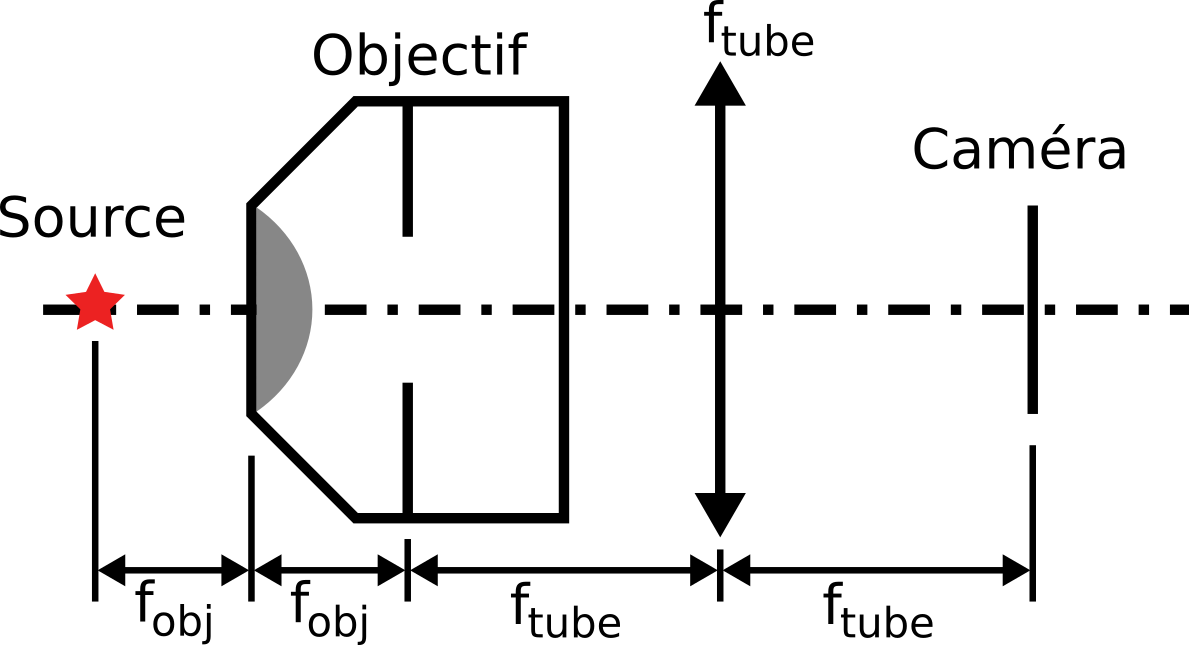
\includegraphics[scale=2.3]{systeme.png}
  \caption{Système optique simplifié du microscope.}
  \label{sys}
\end{figure}
Afin de simuler les observations et les analyses qui seront faites avec le microscope,
une modélisation du mouvement d'une particule a premièrement été effectué sur un scripte Python.
Pour les fins du projet, une seule particule a été suffisante pour
évaluer les paramètres à optimiser, puisque l'objectif est d'estimer une caractéristique propre 
à une particule, sa taille, et non à un regroupement de particules. En guise d'équivalence à la magnification réelle du microscope, 
une taille de pixel effective $P$ a eu besoin d'être posée. Le calcul de cette taille $P$ est obtenue à partir du grossissement $M$ de l'objectif ainsi qu'avec la
focale de la lentille de tube $f_{tube}$. Le grossissement est défini tel que :

\begin{equation}\label{m_1}
  M = \frac{f_{tube}}{f_{obj}},
\end{equation}

où $f_{obj}$ est la longueur focale de la lentille objectif. Le grossissement $M$ connu des lentilles suit
un standard de la \textit{Royal Microscopical Society} (RMS) qui pose $f_{tube}$ à 160 mm
\cite{RMS}. Ainsi, pour avoir le grossissement réel $M_{r}$, il faut convertir avec la 
formule suivante :

% Source A : https://www.microscopyu.com/microscopy-basics/infinity-optical-systems

\begin{equation}\label{m_2}
  f_{1}= \frac{160 \text{ mm} }{M} \Rightarrow M_{r} = \frac{f_{obj}M}{160 \text{ mm} }.
\end{equation}

La taille réelle d'un pixel de caméra $p_r$, d'une valeur de 3.45 µm pour la caméra Zelux CS165MU
mise à disposition pour ce contrat \cite{thorlabs}, peut être convertie en taille effective
avec le grossissement réel :

\begin{equation}\label{pixel}
  P = \frac{p_{r}}{M_{r}} = \frac{p_{r}\;160 \text{ mm}}{f_{obj}M}.
\end{equation}

Pour créer un environnement plus fidèle à la réalité, un fond de bruit
a été rajouté, où les photons émis suivent une distribution de Poisson avec \textit{np.random.poisson}. En raison de la diffraction 
causée par le système optique, la particule a due être simulée
telle qu'elle serait perçue par la caméra dans le montage réel. En fonction des composantes optiques utilisées,
la PSF (\textit{Point Spread Function}) de la particule sur le capteur est décrite par:
\begin{equation}
  PSF(r)=\left(\frac{2J_1(\frac{2\pi \text{NA}r}{\lambda})}{\frac{2\pi \text{NA}r}{\lambda}}\right)^2,
\end{equation}
où NA est l'ouverture numérique de l'objectif, $\lambda$ est la longueur d'onde de la lumière passant à travers
le microscope et r est la distance radiale par rapport à la position de l'émetteur \cite{procedurier}. Ici, $J_1$
est une fonction de Bessel. L'émission des photons dans le temps s'effectue selon une distribution de Poisson:
\begin{equation}
  P(X=k)=\frac{\lambda^k e^{-\lambda}}{k!},
\end{equation}
où $k$ est le nombre d'évènements et $\lambda$ est le nombre moyen d'évènements
survenus au cours d'un intervalle de temps défini (le temps d'acquisition). Numériquement, ceci correspond à effectuer un nombre de simulations
d'émission choisi avec \textit{np.random.poisson} et une valeur $\lambda=400$ arbitraire. La position de chaque photon
émis durant la simulation est déterminée à l'aide de la distribution de probabilité imposée par la fonction d'étalement 
de la particule ($PSF$).

Pour simuler le mouvement d'une particule, on utilise le principe du mouvement brownien.
Le centre d'une gaussienne est placé à la position exacte de la particule, et son écart-type correspond à la probabilité de présence de la particule sur une position x et y, 
relativement proche de la position initiale, après un certain intervalle de temps $\Delta t$. L'écart-type de la gaussienne possède la forme suivante:
\begin{equation}
  \sigma_{diffusion} = \sqrt{2D\Delta t} = \sqrt{2\left ( \frac{k_{B}T}{2\pi \eta r} \right )\Delta t},
\end{equation}
où $D$ est le coefficient de diffusion, $k_{B}$ la constante de Boltzmann, T la température en Kelvin, $\eta$ la viscosité en $Pa\cdot s$, r le rayon de la particule en mètre et $\Delta t$ le temps entre chaque déplacement en secondes. 
Avec une fonction python, il est possible de placer la particule à sa nouvelle position en tenant compte de ces probabilités. Cette opération est répétée successivement pour observer 
le déplacement de la particule, et est testé pour des particules de diamètre de 1 et 10 µm.


Après avoir simulé le mouvement d'une particule, l'analyse a pu être effectuée en utilisant une procédure similaire
à celle qui sera utilisée pour le système réel. Pour chaque image capturée lors de l'acquisition, un \textit{fit}
d'une gaussienne 2D a été effectué avec la librairie \textit{lmfit}. La fonction gaussienne 2D est définie par:
\begin{equation}
  f(x,y)=A\cdot exp\left(-\left[\frac{(x-x_0)^2}{2\sigma_x^2}+\frac{(y-y_0)^2}{2\sigma_y^2}\right]\right)+B,
\end{equation}
où $A$ est l'amplitude et $B$ est le décalage de la gaussienne. À partir de la fonction obtenue, les moyennes en $x$ et en $y$ ($x_0,y_0$) de la gaussienne sont obtenus
pour estimer la position de la particule à cet instant. En effectuant ce processus pour chaque image de l'acquisition,
on a pu obtenir le déplacement général de la particule pour un certain lapse de temps.


Une fois les positions obtenues, il est possible de trouver la valeur du coefficient de diffusion de la particule. 
Pour ce faire, il est nécessaire d'effectuer le calcul du déplacement quadratique moyen. On réalise ce calcul en faisant la moyenne des déplacements de même intervalle. Par exemple, 
la première moyenne sera calculée avec toutes les distances séparant deux positions éloignées d'un intervalle de $\Delta t=1$. De la même manière, la deuxième moyenne sera calculée avec toutes les distances
entre deux points placés à $\Delta t=2$ d'intervalle. On peut modéliser ce calcul par la formule suivante: 
\begin{equation}
  MSD = \frac{1}{N_{\Delta t}} \sum_{i=0}^{N_{\Delta t} - 1} \left( \mathbf{r}(i+\Delta t) - \mathbf{r}(i) \right)^2
\end{equation}
Avec $N_{\Delta t}$ qui est le nombre de paires $i$ disponibles pour un intervalle $\Delta t$ et $\Delta t$ qui varient de 1 jusqu'au nombre de positions (nombre d'images) moins une. 
Une fois les valeurs des MDS trouvés pour chaque déplacement de même intervalle, il est possible de générer un graphique 
des MDS en fonction de la valeur de l'intervalle $\Delta t$. Sur ce graphique, seuls les premiers points seront sélectionnés, c'est-à-dire pour des $\Delta t$ faibles.
Cette procédure est nécessaire pour observer le comportement réel du mouvement, car plus $\Delta t$ est petit, plus il existe de paires disponibles. 
Une régression linéaire est effectuée sur
ces points; c'est la pente de cette régression qui donnera la valeur du coefficient de diffusion $D$ et ainsi la taille de la particule $r$ estimée par notre microscope :

\begin{equation}
  \langle MSD(t) \rangle = 4Dt + 4\sigma_{diffusion}^{2}
\end{equation}
où $D=k_{B}T/2\pi \eta r$.
Les valeurs obtenues par cette procédure comportent toutes une incertitude. L'incertitude sur chaque 
position $x$ et $y$ est donnée par l'écart-type de sa gaussienne:
\begin{equation}
  \Delta x=\Delta y=\sigma_{position}
\end{equation}
Une fois l'incertitude déterminée pour chaque valeur, on veut pouvoir déterminer l'incertitude sur chaque valeur de la MSD. 
Pour ce faire, on propage l'incertitude, par la formule suivante, de chaque position sur la valeur de la MSD  correspondante: 
\begin{equation}
  \alpha =A+B
\end{equation}
\begin{align*}
  A = \sqrt{
    \begin{aligned}
      &\left( 2(x(i+\Delta t) - x(i))\cdot \Delta x(i+\Delta t) \right)^2 \\
      &+ \left( 2(x(i+\Delta t) - x(i))\cdot \Delta x(i) \right)^2
    \end{aligned}
  }
\end{align*}
\begin{align*}
  B = \sqrt{
    \begin{aligned}
      &\left( 2(y(i+\Delta t) - y(i))\cdot \Delta y(i+\Delta t) \right)^2 \\
      &+ \left( 2(y(i+\Delta t) - y(i))\cdot \Delta y(i) \right)^2
    \end{aligned}
  }
\end{align*}

\begin{equation}
  \Delta MSD=\frac{1}{N_{\Delta t}}\sqrt{\sum_{0}^{N_{\Delta t}-1}\alpha, }
\end{equation}
en sachant que $\left ( r(i+\Delta t)-r(i) \right )^{2}=\left ( x(i+\Delta t)-x(i) \right )^{2}+\left ( y(i+\Delta t)-y(i) \right )^{2}$.
On peut tracer une régression linéaire, où l'incertitude sur la valeur de la pente de cette régression est donnée par l'équation \ref{deltad}.
Celle-ci considère qu'il n'y a des incertitudes que sur les valeurs en $y$ (MSD) et que cette incertitude n'est pas constante pour chaque point.
\begin{equation}\label{deltad}
  \Delta D=\sqrt{\frac{\sum_{i=1}^{N}(\Delta MSD_{i})^{2}}{\sum_{i=1}^{N}{(x_{i}-\overline{x})^{2}}}}
\end{equation}
Où $N$ est le nombre d'intervalles considéré. 

Afin de déterminer quels objectifs de microscope considérer pour le produit final, la définition
de la résolution est nécessaire pour la vérification du théorème d'échantillonnage de Nyquist. Soit $d$,
la limite de diffraction pour une source ponctuelle au travers d'une ouverture \cite{video}:
\begin{equation}
  d = \frac{\lambda}{2 \text{NA}},
\end{equation}

où $\lambda$ est la longueur d'onde éclairant l'échantillon observé et NA est l'ouverture numérique de
l'objectif. Cette limite de diffraction est la résolution du système. Ainsi, selon le théorème
de Nyquist, la taille effective d'un pixel de la caméra $P$ dans le plan de l'objet observé doit respecter :

\begin{equation}\label{nyquist}
  P \leq \frac{d}{2} = \frac{\lambda}{4 \text{NA} }.
\end{equation}


Ainsi, pour un système avec $f_{obj}$ \textcolor{red}{ou tube?} et $M$ connus (voir équation \ref{pixel}), il est possible de déterminer si le théorème 
(\ref{nyquist}) est respecté pour une longueur d'onde donnée. Cela a permis de déterminer quelles 
combinaisons de lentille tube, d'objectif de microscope et de source de lumière qui ne sont pas 
sujettes au phénomène d'\textit{aliasing}, conséquence du non respect de Nyquist où l'information
réelle sur l'image est perdue.

Les paramètres déterminants qui seront pris en compte pour la simulation se résument à la longueur d'onde du faisceau d'entrée,
la magnification et l'ouverture numérique de l'objectif, la longueur focale la lentille objectif \textcolor{red}{obj ou tube?}, la taille de la particule ainsi que le 
coefficient de diffusion. Les variations des paramètres ainsi que les équations
développées ont permis de poser l'hypothèse que les paramètres ne s'infuencent pas entre eux et qu'ils peuvent être traités indépendamment.




\section{Résultats \label{resultats}}
\textcolor{red}{rajouter viscosité} Le tableau \ref{tableau_nyq} présente les calculs de chaque côté de l'inégalité (\ref{nyquist}) pour
chaque combinaison de paramètres possibles avec le matériel mis à disposition par le gouvernement local.
Quatres objectifs, tous ayant une paire de $M$ et NA, ainsi que deux sources de lumière pour faire émettre
des photons par les fluorophores dans les échantillons sont disponibles. La valeur de $f_{obj}$ \textcolor{red}{ou tube?} est fixée à 150 mm, sachant que les lentilles offertes sont limitées à cette longueur focale.

\begin{table}[H]
    \centering
    \caption{Résultats des calculs pour $P$ et $d/2$ en fonction des paramètres possibles.}
    \begin{tabular}{|c|cc||c|c|}
    \hline
        $\lambda$ (nm) & $M$ & NA & $P$ (µm) & $d/2$ (µm) \\ \hline\hline
        \multirow{4}{*}{405} & 10 & 0.25 & 0.368 & 0.810 \\ \cline{2-5}
                             & 20 & 0.4  & 0.184 & 0.506 \\ \cline{2-5}
                             & 40 & 0.65 & 0.092 & 0.312 \\ \cline{2-5}
                             & 60 & 0.85 & 0.061 & 0.238 \\ \hline
        \multirow{4}{*}{375} & 10 & 0.25 & 0.368 & 0.750 \\ \cline{2-5}
                             & 20 & 0.4  & 0.184 & 0.469 \\ \cline{2-5}
                             & 40 & 0.65 & 0.092 & 0.288 \\ \cline{2-5}
                             & 60 & 0.85 & 0.061 & 0.221 \\ \hline
    \end{tabular}
\label{tableau_nyq}
\end{table}

Les résultats obtenus avec la simulation pour certains paramètres sont présentés dans le tableau \ref{results} ci-dessous. Les valeurs des paramètres $\lambda$,
$M$ et NA sont les mêmes que ceux présentés dans le tableau \ref{tableau_nyq}. Encore une fois, $f_{obj}$ \textcolor{red}{ou tube?} est fixée à 150 mm pour les simulations. La taille correspond au diamètre
de la particule.
\begin{table}[H]
  \centering
  \caption{Valeurs obtenues pour le coefficient de diffusion $D$ et la taille de la particule pour certains paramètres de simulation.}
  \begin{tabular}{|C{0.5cm}|cc|C{0.6cm}|C{1.3cm}||C{1.1cm}|C{1.1cm}|}
  \hline
      \multicolumn{5}{|c||}{Paramètres} & \multicolumn{2}{c|}{Résultats} \\ \hline
      $\lambda$ (nm) & $M$ & NA & Taille réelle ($\mu m$) & $D_{vrai}$ ($\mu m^2/s$)  & $D_{est}$ ($\mu m^2/s$)  & Taille estimée ($\mu m$)\\ \hline\hline
      405 & 10 & 0.25 & 1 & 0.10981691 & 0.065 $\pm$ 0.004 & 0.60 $\pm$ 0.04 \\     
      405 & 20 & 0.4 & 1 & 0.10981691 & 0.087 $\pm$ 0.002 & 0.79 $\pm$ 0.02 \\
      405 & 40 & 0.65 & 1 & 0.10981691 & 0.066 $\pm$ 0.002 & 0.60 $\pm$ 0.02 \\
      405 & 60 & 0.85 & 1 & 0.10981691 & 0.105 $\pm$ 0.002 & 0.96 $\pm$ 0.02 \\
      375 & 20 & 0.4 & 1 & 0.10981691 & 0.085 $\pm$ 0.003 & 0.78 $\pm$ 0.03 \\
      405 & 20 & 0.4 & 10 & 0.010981691 & 0.0166 $\pm$ 0.0008 & 15.1 $\pm$ 0.7 \\
\hline
      \end{tabular}
\label{results}
\end{table}




\section{Discussion}
Les résultats des deux dernières colonnes du tableau \ref{tableau_nyq} laissent conclure que les paramètres choisis respectent tous le critère de Nyquist.
De plus, l'impact des paramètres sur la résolution semblait indiquer qu'un plus grand $M$ (et NA)
ainsi qu'une plus petite longueur d'onde étaient à préconiser pour minimiser $d$. La simulation suivant
le modèle mathématique a vérifié cela. Cette conclusion n'élimine donc aucun objectif et tous les paramètres du tableau \ref{results} peuvent 
être considérés pour les prochaines analyses.

Les simulations effectuées pour la deuxième et la cinquième rangées du tableau \ref{results}, soit pour un faisceau entrant ayant une longueur d'onde de 405 nm ou de 375 nm,
ont menées à une incertitude relative sur la taille de la particule de 21 $\pm$ 2 \% et 22 $\pm$ 3 \%, respectivement. Ceci correspond à une différence extrêmement minime, surtout en 
considérant l'ordre de grandeur des erreurs. Leurs incertitudes sont proportionnelles à celles obtenues pour la taille de la particule et sont aussi très similaires. Les valeurs de $d/2$ obtenues dans le
tableau \ref{tableau_nyq} soutiennent le fait qu'une longueur d'onde plus petite améliore la résolution, mais cette corrélation n'est pas évidente dans les résultats
obtenus avec la simulation. Par conséquent, la complication de l'alignement associée à l'usage d'un laser dans le domaine ultraviolet, beaucoup plus importante, renforce plutôt le choix d'utiliser un faisceau de $\lambda=405$.

Les quatres premières rangées du tableau \ref{results} permettent de comparer l'effet de la magnification et de l'ouverture numérique sur la taille estimée et son incertitude associée. Pour les paires de [$M$, NA] 
suivantes: [10, 0.25], [20, 0.4], [40, 0.65] et [60, 0.85], les erreurs relatives obtenues pour la taille de la particule sont respectivement: 40 $\pm$ 4 \%, 21 $\pm$ 2 \%, 
40 $\pm$ 2 \% et 4 $\pm$ 2 \%. L'erreur relative presque négligeable sur la taille obtenue avec une objectif ayant [60, 0.85] semble prédire qu'une augmentation de la magnification et de l'ouverture numérique
améliore fortement la performance du microscope. Il est aussi important de noter qu'une magnification trop grande pourrait porter problème et affecter la justesse des résultats si le champ
de vision résultant est réduit au même ordre de grandeur que les particules observées. Le cas échéant, la particule pourrait facilement se déplacer hors du cadre de l'image, ce qui rendrait l'analyse de
son déplacement beaucoup plus difficile. Cependant, pour l'objectif [60, 0.85], la magnification est encore beaucoup trop petite pour considérer cet enjeu. L'objectif choisi est donc [60, 0.85].

Il est aussi important de s'assurer que l'analyse du déplacement soit aussi performant pour des tailles de particules variées, d'où l'utilité du test 
effectué pour une particule de 10 $\mu m$. L'erreur relative pour cette simulation est de 85 $\pm$ 7 \%. En comparant cette erreur à celle obtenue pour le test ayant les mêmes paramètres mis à part la taille (deuxième
rangée du tableau \ref{results}), on voit que l'erreur est beaucoup plus importante pour la particule ayant un plus grand diamètre. Cette différence peut être due à des variations dans le \textit{fit} gaussien utilisé pour localiser
la particule à chaque image. Puisque la particule est plus large, la fonction gaussienne s'étale, ce qui augmente la possibilité que le centre de celle-ci ne s'aligne pas
avec le centre réel de la particule. L'analyse a tout de même retrouvée une taille estimée du même ordre de grandeur que la taille réelle, ce qui est convenable pour le contexte du projet.

\printbibliography

\clearpage

\section{Annexes}

\subsection{Preuve de correction par Antidote}

\clearpage


\end{document}
